\subsection{Survey Geometry}\label{subsec:geometry}


The vehicle moves at speed v = 1.0 m/s along straight legs that cross a straight cable at an incidence θ (Figure 1a). Two tri-axial fluxgates are mounted at the water line on the vehicle's lateral axis, UNO on the port side and DUO on the starboard side, separated by the baseline b = 1 m. For each sensor we use a local CPA frame: the origin is the point of its track directly above the cable, x̂ is the horizontal normal to the cable, ŷ points along the cable and ẑ points down (Figure 1b). The cable then lies at x = 0, z = d, where d is the standoff.

A sensor that crosses the cable at time t\textsubscript{c} has horizontal distance x = v(t − t\textsubscript{c}) sin θ from the cable at time t. Every field quantity below depends on x only through the ratio x/d, so we use the normalised coordinate

\[
\tau=\frac{x}{d}=\frac{v\,(t-t_c)\sin\theta}{d}=\frac{t-t_c}{T_s},\qquad T_s=\frac{d}{v\sin\theta}. \tag{1}
\]

τ counts CPA distances, and T\textsubscript{s} is the time the sensor takes to move one CPA distance across the cable; at θ = 50° and v = 1 m/s it is 2.6 s for d = 2 m and 5.2 s for d = 4 m. T\textsubscript{s} is the time scale of every matched template, and we call it the template scale. A leg that starts and ends at the lateral distance A from the cable covers \textbar x\textbar{} ≤ A, i.e.~\textbar τ\textbar{} ≤ K 

with

\[
K=\frac{L}{d},\qquad L=A\ \text{for a snake leg}. \tag{2}
\]

L is the half-length of the pass measured across the cable. With the snake amplitude A = 6 m used in closed loop and d = 2--4 m, K = 3--1.5: a snake leg sees only a few CPA distances on each side of the crossing.

\begin{figure}
\centering

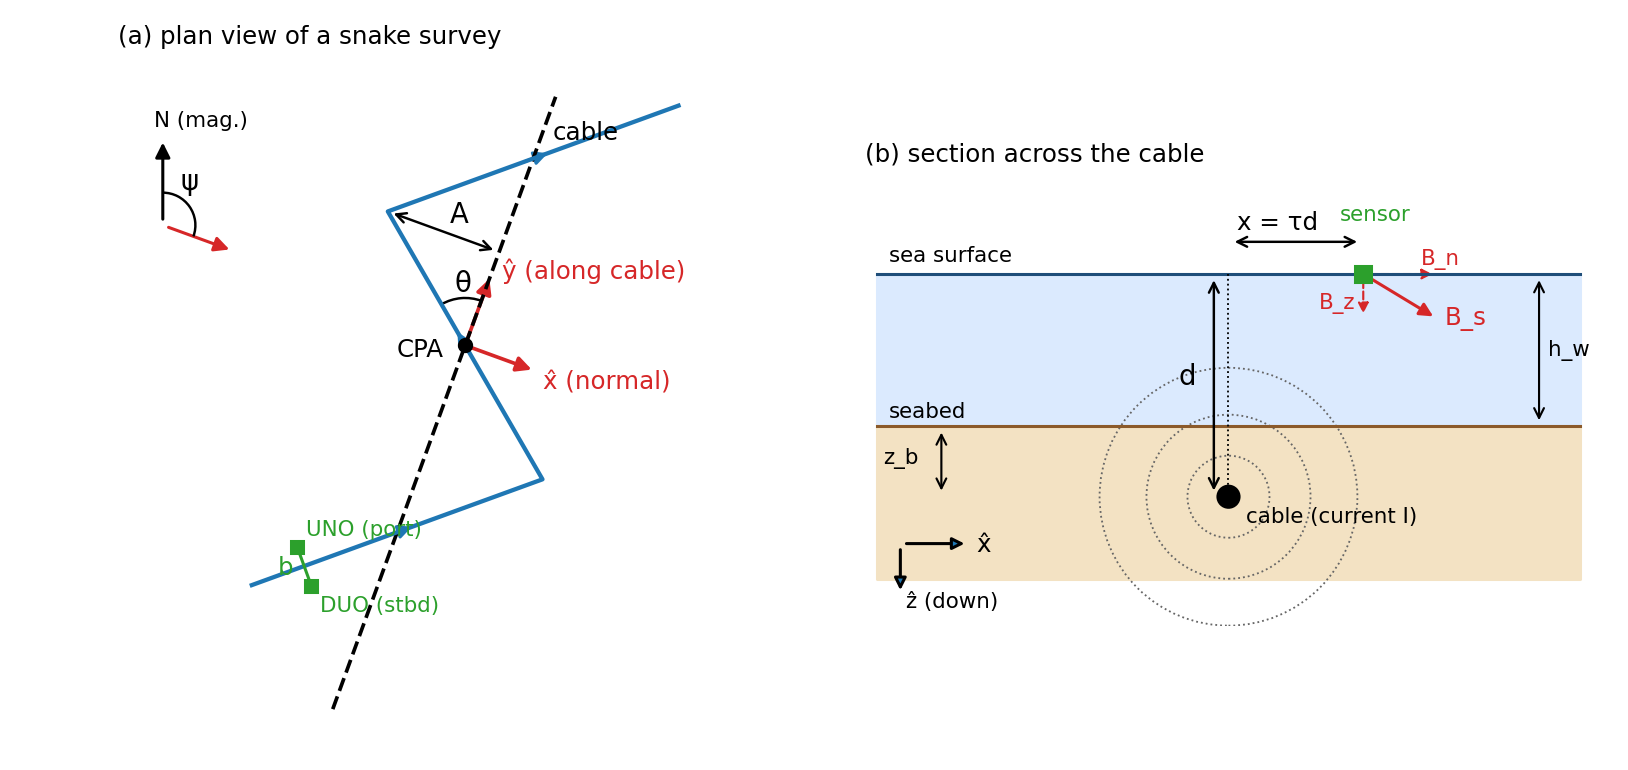
\includegraphics[width=0.98\textwidth,height=\textheight]{paper/sec_2_geometry_signal_model/figures/F1_geometry.png} 

\caption{Survey geometry. (a) Plan view of a snake survey: cable(dashed), legs crossing it at incidence θ with amplitude A, CPA frame (x̂ normal, ŷ along the cable), the two sensors UNO and DUO separated by the baseline b, and the angle ψ from magnetic north to the cable normal. (b) Section across the cable: the sensor at the surface, the cable at standoff d below it (burial depth z\textsubscript{b} below a seabed at water depth h\textsubscript{w}), the normal coordinate x = τd, and the azimuthal cable field B\textsubscript{s} with its normal and vertical components B\textsubscript{n} and B\textsubscript{z}.}
\end{figure}